\chapter{Transforming Semantic Notes into Semantic Blog Posts}
\label{ch:semblogging}

\begin{flushright}
 \textit{Based on ``Linking Semantic Personal Notes'' \cite{Dragan2010a}\\published at the Workshop on Knowledge Injection into and Extraction from Linked Data (KIELD~2010~co-located~with~EKAW~2010)}
\end{flushright}

In the previous two chapters we showed how Semantic Web technologies are available both on the desktop and of course on the Web, and how the two networks of linked data can be connected. SemNotes, a semantic note-taking tool for the Semantic Desktop, described in Chapter \ref{ch:semnotes}, shows how new data can be created and seamlessly integrated with existing semantic information from the desktop. Chapter \ref{ch:sdwod} describes an algorithm for automatically connecting desktop resources to their Web aliases, bridging the gap between the desktop and the Web in regards of semantic data, opening up the possibility of augmenting desktop data and building personalised desktop services. 

In this chapter we present a use case, and a proof of concept system which builds on our previous work in order to support easy publishing and sharing of semantic personal notes taken with SemNotes as Linked Data.
Our approach can be used to publish any kind of information from the desktop to the Web, enabling integration of small chunks of personal knowledge into the Web of Data.
This use case illustrates a solution to the second research question \textbf{Q 2.} from Section \ref{sub:question}, \emph{How to expand the scope of the Semantic Desktop into the realm of the Web of Data, to enhance the user experience and benefit?}, more specifically, to the second and third sub-questions \textbf{Q 2.2.} --- \emph{How to use the Web information found related to a desktop resource?}, and \textbf{Q 2.3.} --- \emph{How to make desktop data available online safely?}

\section{Introduction}
\label{sec:introduction}

Semantic Web technologies are deployed in various domains and applications, both on the desktop and on the Web.
While these two domains share compatible representation models (RDF(S)/OWL), there is still a gap between data from the Web and the desktop. We showed in the previous chapter how finding Web aliases for Semantic Desktop resources enables us to bridge this gap. This solution is however unidirectional --- it only solves connection from the desktop to the Web, and not the reverse, from the Web to the desktop. It can be argued that accessing desktop information from the Web is not necessary, or not safe, or that the risks exceed the benefits. However, sharing desktop information online has many possible use cases, and does not necessarily involve making private information public. 

One such use case of sharing desktop information and realising better integration of personal data with online data, is described in this chapter. We present an approach for publishing personal notes from the desktop (using SemNotes and Semantic Desktop technologies) to the Web of Data (using the Linked Data principles). Our goal is to publish this data online without losing the personal context established on the desktop through the links from the notes and the related desktop resources.
Our approach consists of two main steps: 
\begin{enumerate}
 \item preparing the desktop data for sharing, 
 \item publishing it online. 
\end{enumerate}
In addition, it requires two prerequisite steps, which are supported by previous work: 
\begin{itemize} 
 \item the note-taking process and annotation of the note (adding the context) which was presented in Chapter \ref{ch:semnotes}, and 
 \item the identification of Web URIs which represent the same real-world thing as the desktop resources that belong to the context of a note, which was presented in Chapter \ref{ch:sdwod}. 
\end{itemize}

Our contribution consists of the process for publishing personal information from the desktop to the Web following the Linked Data principles \cite{BernersLee2006}, and a system implementation that allows sharing of semantic personal notes as semantic blog posts, interlinked with existing information from the Web of Data. 
The publication process must follow the Linked Data principles, while at the same time protecting sensitive private data from being shared unwillingly, and maintaining the meaningful relations in the process.


The semantic notes taken with SemNotes constitute the personal information that we want to publish as Linked Data. They are semantically linked to local resources mentioned in their content, like people, projects or other notes. If the notes were directly published online, the relations that enrich them would be lost and the links they contain would be broken, because they point to local URIs not available outside of the desktop. The same objects often exist within the Web of Data, therefore the note links to them can be recreated in the publishing process. Before the note is published, our system searches for existing public Web aliases for the local resources. They are then used to substitute the local private data referenced in the text --- the links are changed to point to the Web resource. In this way, the published links are valid, the meaning of the link is preserved (as referring to the same entity) and the private information is protected. The system then publishes the notes online as blog posts 
taking care of the transformations required from desktop ontologies to Web ones, according to the mappings devised in Chapter \ref{ch:sdwod}.

In line with the two-step process mentioned above, our system has two modules, one working on the desktop and the second one online. First, the desktop part handles the preparation of the notes for publishing, using the Web aliases identified by the service described in the previous chapter, substituting them for the local ones, as well as the transformation required from desktop ontologies to Web ones. This module is invisible to the user, except for the \emph{Publish} button shown in the user interface of SemNotes. Then, the Web part publishes the transformed notes as Linked Data in accordance with the Linked Data publishing principles.

The solutions provided by most existing systems fall into two categories: \begin{inparaenum}[(i)] \item desktop applications that involve publishing the actual local resource information together with the note, or \item online applications that do not have access to desktop data relevant to the user. \end{inparaenum} The first category, represented by tools like SemiBlog \cite{Moeller2005} or SemBlog \cite{Takeda2005}, is not optimal when dealing with resources that contain sensitive private information. Services like Zemanta\footnote{\url{http://www.zemanta.com}}, from the second category, have access to various online resources, but not to the personal context of the user.
Also they miss the personal touch of desktop-based applications.


\section{From Note-Taking to Weblogging}
\label{sec:reqsemblog}

Two characteristics of blog posts which are relevant to this use case are: 
\begin{itemize}
 \item their topics are of interest to the author and thus are very likely to have references to things also present on the desktop (e.g. people, events); 
 \item the context consists of the references made in their content, such as places, projects, or other blog posts.
\end{itemize}

However, not all blog posts start by being a blog post. Some are just ideas or impressions jotted down for later, in one's preferred desktop note-taking application. Nevertheless, some of these notes do become posts after polishing and refining, especially as some notes might require further investigation before they can be published (e.g. when writing on a technical subject). Examples include notes taken at presentations, ideas on topics of interest written down at times when blogging is not possible (attending a meeting or lack of Internet connection).

Tools from the Semantic Desktop, like SemNotes, provide means to enhance these notes locally, by interlinking them with other desktop data --- the contacts in the address book, the events from the calendar application, the projects worked on, the music listened to. 
For example, a note about an upcoming concert can be linked to the performing artist which is in turn linked to the music files of that artist and pictures from earlier shows stored in a desktop photo application.
Such annotations give context to the note and should be preserved when the note is published as a blog post on the Web, since it enables serendipitous browsing and information discovery, through the relevant additional links they contain.

Currently, personal notes, even the ones semantically enriched using Semantic Desktop applications, must be published as blog posts by being manually copied into a blogging tool.
In this way, any additional semantic information available on the desktop is lost or, if copied, leads to broken references as they point to the local resources which are not accessible outside of the desktop.
The note-taking to publishing process is sometimes cut short by using the drafting functionality offered by some systems like WordPress or Blogger, so that users can directly take the notes in the blogging tool, usually online, thus replacing the desktop note-taking application completely. However, using online tools deprives the user from having the personal context added to the blog post, since desktop information cannot be easily integrated in Web-based services.

In order to enable a better transition from personal notes to blog posts, or simply to Web-based information available to others (for example, meeting notes published in a company intranet or lecture notes shared between students of the same class), we defined a list of requirements that a system for publishing semantic personal data online should fulfil:
\begin{description}
 \item[R1.] Publish the complete desktop data on the Web without losing any relevant information, including metadata and context (e.g. tags, relations, identifiers);
 \item[R2.] Protect any machine readable and private data that might be unwillingly included in the context being transferred\footnote{The protected data does not include the actual text to be shared as it is a conscious decision to publish it, taken explicitly by the user};
 \item[R3.] Publish the note according to the Linked Data principles and describe it using popular ontologies; 
 \item[R4.] Enable object-centred sociality by establishing connections between data published by different users.
\end{description}


\section{Overview of the Process and Prerequisite Steps}
\label{sec:sembloggingapproach}

We propose an approach that enables the publishing and sharing of personal notes by extending the functionality provided by SemNotes, and by using the Web of Data aliases found for desktop resources. The process consists of two steps: 
\begin{enumerate} 
 \item transformation, and 
 \item publication. 
\end{enumerate}
In the first step, the note is transformed locally for publication, and private local data is replaced with public references.
In the second step, the transformed note is published online.

The system requires a dedicated server, where the resources referenced and the tags assigned are shared between the notes of all users, to add a social aspect. Also, rather than trying to determine which of the many possible Web aliases found for a desktop resource is authoritative, we let the server create equivalent public resources and connect all the aliases to them. We also used the server for publishing the notes, although this can be replaced by any other blogging platform.

The first prerequisite step --- note-taking and annotation of the note with the relevant desktop resources --- must be performed before any actual sharing of notes can be done. The annotation is done semi-automatically and is an existing feature in SemNotes. 

The second prerequisite step consists in finding Web resource for each of the desktop entity linked to the note that is about to be published. This step is executed by a desktop service which implements the two-part algorithm detailed in the previous chapter, the blocking pass using Sindice to retrieve possible candidates and filtering the list by the score returned by the matching algorithm. The local service has access to, and uses all the information available on the desktop about a resource to identify only exact matches for it. The aliases which are found for the desktop resources are saved by creating a \verb|pimo:hasOtherRepresentation| link in the local repository between the desktop resource and the Web one.


\section{System Implementation Details}
\label{sec:sembloggingsystem}

Based on the process described above, the system is divided between its local part and its remote part, as shown in Figure \ref{fig:semblogsystem}. The local part handles local \emph{private} data, while the remote one handles online \emph{public} data. 
\begin{figure}[htb]
  \begin{center}
    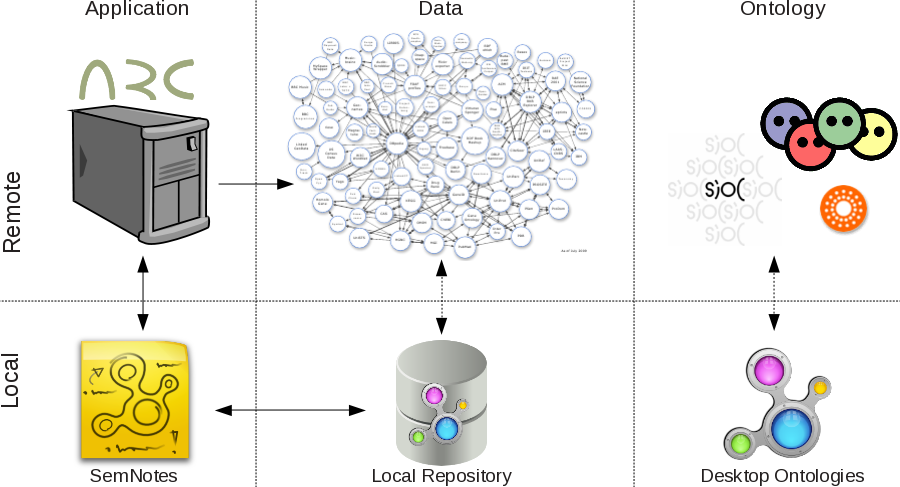
\includegraphics[width=0.8\linewidth]{chapters/core/img/system}
    \caption{Overview of the semantic publishing system.}
    \label{fig:semblogsystem}
  \end{center}
\end{figure}
The separation between them extends over three layers: ontology, data and application.
On the \emph{ontology} layer, the NEPOMUK desktop ontologies are used locally, while popular Web vocabularies are used on the server-side. These ontologies are used to describe the \emph{data} exchanged between the applications. Desktop data is stored in the local NEPOMUK repository, while Web data is distributed. Finally, on the \emph{application} layer, the local component is an extension to SemNotes that provides publishing functionality for notes, and the remote component is a server that hosts and publishes online the notes received.

The first step of the process --- transformation --- is executed on the local side, by an extension of the SemNotes application. Then, the publication step is done by the server, which receives information from the desktop and publishes the note, as we will describe next. The two application components, the communication between them, and the data translation process are described in detail below.

\subsection{Ontologies}

Although both the Semantic Desktop and the Semantic Web use the same representation languages, i.e. RDF(S)/OWL, they use different vocabularies to describe their data. This vocabulary gap makes data integration difficult.

The NEPOMUK project defines a set of desktop ontologies to describe its data.
SemNotes uses these ontologies to represents personal notes as instances of \verb|pimo:Note| and are linked to the \verb|pimo:Thing|s they mention by the relation \verb|pimo:isRelated|. 

When a desktop resource is found to represent the same real world entity as a Web resource, the relation is stored on the desktop as \verb|pimo:hasOtherRepresentation|. This property is recommended by the PIMO specification as desktop equivalent to the \verb|owl:sameAs| relation, although without the formal semantics that the latter provides. We also use the property \verb|pimo:hasOtherRepresentation| to store the remote URL of a note when it is published. If the note changes on the desktop after publication, the property is replaced with \verb|pimo:hasDeprecatedRepresentation|.

While well-suited to represent desktop information, these ontologies are not used, so far, on the Web. However, numerous vocabularies have emerged for describing semantic data published online. Such ontologies have now been widely adopted and are recommended as best practices when publishing data on the Web \cite{Bizer2007}. 

Consequently, while representing similar objects, the two sets of vocabularies must be aligned so that on the one hand, desktop information can be moved to the Web and understood by usual Semantic Web applications that rely on the aforementioned vocabularies, and on the other hand, Web information could be understood and imported by Semantic Desktop applications. In order to enable interoperability between the desktop and the Web, we defined mappings between the sets of ontologies. The mappings create appropriate subclasses or subproperties of the relevant concepts from the chosen vocabularies.

SIOC is probably the most widely used vocabulary for interlinking social media within the Web of Data.
There are already many tools for creating and using SIOC data \cite{Bojars2008}.
This is why we chose to represent the \verb|pimo:Note|s as \verb|sioc:Post|s when they are published online with our system. The rest of the desktop resources are also transformed into concepts from the vocabularies listed above (see Table \ref{tab:classmappings}), the mappings being published at \url{http://rdfs.org/sioc/nepomuk}.
\begin{table}[htb]
\centering
\ra{1.3}
\begin{tabular}{@{}rcl@{}}
\toprule
Class && Subclass of \\ 
\midrule

\verb|pimo:Note| && \verb|sioc:Post| \\

\verb|nao:Tag| && \verb|sioct:Tag| \\

\verb|pimo:Person| && \verb|foaf:Person| \\

\verb|pimo:Project| && \verb|doap:Project| \\

\verb|pimo:Event| && \verb|ical:Vevent| \\

\bottomrule
\end{tabular}
\caption{Sample of the mapping between classes.}
\label{tab:classmappings}
\end{table}
The note's properties, like title, creation and last modification time, are translated to the appropriate Dublin Core properties: \verb|dcterm:created|, \verb|dcterms:modified| and \verb|dcterms:title|. The tags associated locally with the notes are transformed into \verb|sioct:Tag|s associated with the published post using the \verb|sioc:topic| property. Table \ref{tab:propmappings} lists the proposed mappings for properties\footnote{Although \texttt{nao:lastModified} and \texttt{dcterms:modified} do not have the same semantics, defining subproperty relations between them is acceptable.}.

\begin{table}[htb]
\centering
\ra{1.3}
\begin{tabular}{@{}rcl@{}}
\toprule
Property && Subproperty of \\ 
\midrule

\verb|nao:prefLabel| && \verb|rdfs:label| \\

\verb|nao:created| && \verb|dcterms:created| \\

\verb|nao:lastModified| && \verb|dcterms:modified| \\

\verb|nao:hasTag| && \verb|sioc:topic| \\

\verb|pimo:isRelated| && \verb|sioc:related_to| \\

\bottomrule
\end{tabular}
\caption{Sample of the mapping between properties.}
\label{tab:propmappings}
\end{table}


\subsection{Server Schema}

In order to publish the resources with a consistent URI scheme, we defined patterns for naming the objects published from the desktop on the Web. In the schema definition, we apply several Linked Data patterns described in \cite{Dodds2010LDPBook}: 
\begin{itemize} 
 \item patterned URIs --- for all the entities, to make them more human readable; 
 \item proxy URIs --- for the server URIs, to group multiple Web aliases;
 \item equivalence links --- for the resources related to the notes, to unify various sources; 
 \item natural keys --- in the tag URIs. 
\end{itemize}

For each note the server generates a new unique identifier \verb|id| which is used to create the note's URI in the form: \verb|http://notes.server/note/id|.

According to the proxy URIs identifier creation pattern, we generate new URIs for the resources related to the notes. This ensures that the publishing process is consistent and avoids having to choose among several Web aliases a resource could have. Like the notes, each resource has a unique identifier on the server, which is used to create the resource URI according to the following format: \verb|http://notes.server/resource/id|. Resources are shared by all the notes that link to them, which increases the interlinking and the consistency of the data. For each resource, the server keeps internally a list of Web aliases using \verb|owl:sameAs| links.

Tags are considered a particular type of resources, and are also shared on the server. The specific format for the URI: \verb|http://notes.server/tag/label|, differentiates them from regular resources. The label of the tag acts as a unique identifier, and is case sensitive. They are created on the fly, and are persisted when they are used for the first time.


\subsection{Transformation of the Notes for Sharing}

The first step of the process consists of preparing the note for publishing. In this phase all the relevant information about the note is included in the content, specifically the title, creation and last modification time, the tags and the referenced resources. This transformation is necessary, so that less information, specifically only the HTML content of the note is sent to the server, and not the entire RDF graph describing the note. Although the content is already stored as HTML, to include all the metadata about the note, it has to be enriched with RDFa before being posted to the server.

The preparation step is done on the desktop side, by the added extension to SemNotes. 
To include the referenced resources in RDFa, we need to know their server URIs. Therefore the application needs to communicate with the server to retrieve several URIs: 
\begin{itemize}
 \item the URI for the new note to be published, and 
 \item the server URI for each resource referenced by the note. 
\end{itemize}

In case the note has already been published, the user can overwrite the old post (on the Web) or create a new one. Depending on this choice, a new URI is requested from the server, or the existing one is used (that was saved in the local repository when the note was previously published). 

The referenced resources are shared by all the published notes, therefore the server must create the URI for a resource only if it has not been created before. To decide whether a local resource already has a server URI created, the list of Web aliases found for it on the desktop in the second prerequisite step of the process, is sent to the server (see JSON data in Listing \ref{lst:messagetoserver}). If a resource with a matching type and an overlapping list of aliases exists, the server reuses it, otherwise it creates a new one and saves the information about it in its own RDF repository. On the server, the URI aliases are saved as \verb|owl:sameAs| as it is customary for Linked Data. The server URIs for the note and the resources are also stored on the desktop for reuse, as \verb|pimo:hasOtherRepresentation|.
\lstset{
	caption={JSON formatted message sent to the server.}, 
	label=lst:messagetoserver,
	language=js
}
\setlength\parindent{0in}
\begin{minipage}[t]{\linewidth}
\begin{lstlisting}
{
   "id" : "",
   "resources": [
   {
      "id": "nepomuk:/res/bfcdcd1a-4898-492f-940b-4cc4c67799a7",
      "type": "mo:MusicArtist",
      "uris": [
         "http://dbpedia.org/resource/Scorpions_(band)",
         "http://musicbrainz.org/artist/c3cceeed-3332-4cf0-8c4c-bbde425147b6"
      ]
   }
   ]
}
\end{lstlisting}
\end{minipage}
\setlength\parindent{0.21in}

\lstset{
	caption={Server reply with the server URIs for the resource aliases sent.}, 
	label=lst:serverreply,
	language=js
}
\setlength\parindent{0in}
\begin{minipage}[t]{\linewidth}
\begin{lstlisting}
{
   "note":{
      "uri":"http://notes.server/note/4baccab834e20",
      "resources":[
         {
            "local":"nepomuk:/res/bfcdcd1a-4898-492f-940b-4cc4c67799a7",
            "uri":"http://notes.server/resource/4bacca84ca8bb"
         }
      ]
   }
}
\end{lstlisting}
\end{minipage}
\setlength\parindent{0.21in}

In the case when no Web aliases are found for a desktop resource that is related to a note, and thus the list of aliases sent to the server is empty, a new resource is created on the server with the specified type, but without any information attached to it. The server URI is saved on the desktop as \verb|pimo:hasOtherRepresentation| of the resource, and will be available for reuse when other notes related to the same object are published by the same user. However, this resource will not be shared between notes published by different users. If at a later stage a Web alias is found for the desktop resource, it will be added to the resource already created on the server, thus enabling it to be linked to by multiple users.

The communication between SemNotes and the server is done with a single REST call, in order to minimise network delays. The reply contains the newly created URI for the note, if one was required, as well as a list of server URIs for the resources (see JSON data in Listing \ref{lst:serverreply}). The communication between the desktop side and the server is shown in Figure \ref{fig:semblogsequencediag}. 

Using the information received from the server, the note content is enriched with RDFa. The metadata about the note, like type, creation and last modification times and the tags, is added in \verb|meta| tags in the \verb|head| of the HTML page. RDFa is added to the \verb|title| tag and in the \verb|body|, to the links. Listing \ref{lst:rdfa} shows the content of a note prepared for publishing.

\begin{figure}[htb]
  \begin{center}
    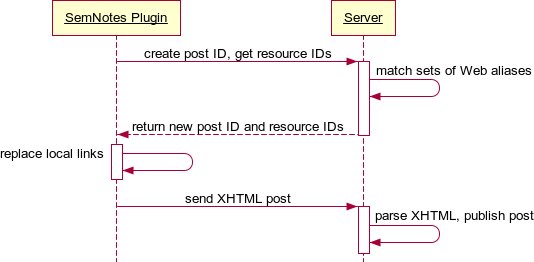
\includegraphics[width=0.85\linewidth]{chapters/core/img/sequencediagram}
    \caption{Sequence diagram for the communication with the server.}
    \label{fig:semblogsequencediag}
  \end{center}
\end{figure}

\lstset{
	caption={RDFa-annotated XHTML content of note.}, 
	label=lst:rdfa,
	language=htmlrdfa
}
\setlength\parindent{0in}
\begin{minipage}[t]{\linewidth}
\begin{lstlisting}
<!DOCTYPE html PUBLIC '-//W3C//DTD XHTML RDFa 1.0//EN' 
                      'http://www.w3.org/MarkUp/DTD/xhtml-rdfa-1.dtd'>
<html about="http://notes.server/note/4baccab834e20">
    <head>
        <meta content="sioc:Post" property="rdf:type"/>
        <meta rel="sioc:topic" href="http://notes.server/tag/concert"/>
        <title property="dc:title">concert sunday</title>
    </head>
    <body>
        <a rel="sioc:is_related"
             href="http://notes.server/resource/4bacca84ca8bb">scorpions</a> concert on sunday was great ...
    </body>
</html>
\end{lstlisting}
\end{minipage}
\setlength\parindent{0.21in}


\subsection{Publication Step}

After the preparation step, which takes place on the desktop side, the RDFa enriched content is sent to the server via another REST call. The publication step of the process only handles public data. When the content is received it is parsed and the server extracts the contained RDF triples and stores them in its repository. The content (as it is received) is also stored.

The server implementation uses ARC2\footnote{\url{http://arc.semsol.org}}, as it provides out of the box RDFa parsing and an RDF repository. It is easily deployable due its minimal setup requirements (a PHP enabled Web server and a MySQL database), thus making our system easily deployable as well.

All server URIs are dereferenceable, as required by the Linked Data principles. For notes, the URI redirects to the RDFa annotated HTML page containing the note itself (as shown in Figure \ref{fig:views} (i)), the URI of the note being the URL of this page. For the linked resources, the URI is also dereferenceable and provides RDFa information about itself, linking to the known existing Web aliases of the same resource. The description also includes a list of backlinks to all the notes that reference the resource (see Figure \ref{fig:views} (ii)). The page for a tag will contain backlinks to all the notes tagged with it.

The RDFa annotated page for the note is generated on the user's desktop by the SemNotes plugin, as we have seen in the previous step, while the page describing each resource and tag is generated on the fly, by the server, when the URI is requested.

\begin{figure}[tb]
\begin{minipage}[b]{0.49\linewidth}
\begin{flushleft}
    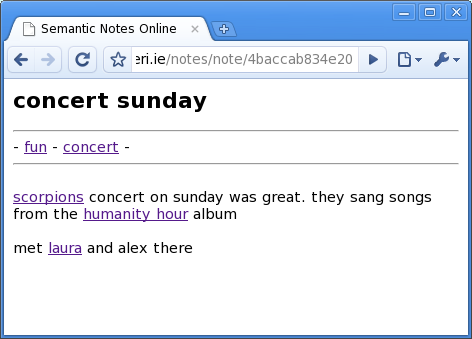
\includegraphics[width=0.97\linewidth]{chapters/core/img/noteview}
\end{flushleft}
\end{minipage}
\begin{minipage}[b]{0.49\linewidth}
\begin{flushright}
    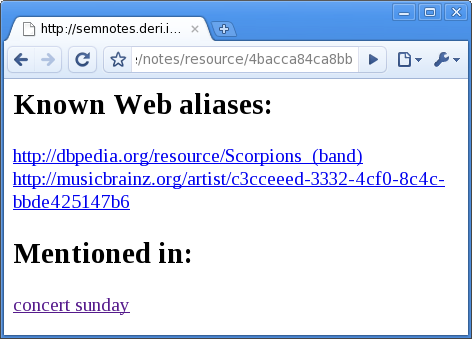
\includegraphics[width=0.97\linewidth]{chapters/core/img/resourceview}
\end{flushright}
\end{minipage}
\caption{Online view of a note (i) and a resource (ii).}
\label{fig:views}
\end{figure}


\section{Conformance with the Initial Requirements}
\label{sec:evaluationsemblog}

When establishing the specifications of the framework, we identified four main requirements (Section \ref{sec:reqsemblog}).
Our proposed implementation conforms with them as follows.

\emph{\textbf{R1}: Publish the complete desktop data on the Web without losing any relevant information, including metadata and context (e.g. tags, relations, identifiers).}\\
By translating existing desktop data surrounding the note to RDF and putting it online, available as RDFa, the entire information available on the desktop side is made available on the Web for further reuse.
In addition, all information from the original note-taking tool, including title, tags, etc. is publicly made available on the Web.

\emph{\textbf{R2}: Protect any machine readable and private data that might be unwillingly included in the context being transferred;.}\\
By replacing the private desktop data with equivalent public Web data, we protect the former. On the desktop there is a lot of private information stored about resources, like the email address or telephone number for people, or the list of attendees of an event. When the person or event is linked to a note that is afterwards published online, such private information is not exported, because the reference to the local resource is replaced by a reference to already public Web data representing the same thing. In this manner, the context of the note being published is preserved, but the private details are not exposed.

\emph{\textbf{R3}: Publish the note according to the Linked Data principles and describe it using popular ontologies.}\\
Our system publishes notes on the Web using the Linked Data principles. Each note and connected resource, has its own URI, which is made dereferenceable, while distinguishing information resources and non-information resources.
In addition, while original desktop data is provided using ``desktop ontologies'', the published information is made available using FOAF, SIOC, Dublin Core, etc. and the mappings have been validated through Vapour\footnote{\url{http://vapour.sourceforge.net/}}.

\emph{\textbf{R4}: Enable object-centred sociality by establishing connections between data published by different users.}\\
Since resources and tags are shared between users, notes can be browsed serendipitously through shared connections, or tags. 
This enables ``object-centred sociality'' \cite{KnorrCetina1997}, since people can interact around these shared tags and topics, such as projects or people that they have in common.
Depending on the destination of the publishing process, there is the possibility of having private notes, yet still accessible online by registered users only.


\section{Related Work}
\label{sec:relatedworksemblog}

Semantic blogging was introduced by \cite{Cayzer2003}, and since then has received much interest. Later \cite{Karger2004} described semantic blogging in the context of the Semantic Web with Haystack. So far, existing systems for semantic blogging fall into two categories: 
\begin{itemize}
 \item desktop applications that involve publishing the actual local resource information together with the blog post, or
 \item online applications that do not have access to desktop data relevant to the user. 
\end{itemize}

The tools in the first category, like SemBlog \cite{Takeda2005} and SemiBlog \cite{Moeller2005}, have the advantage that users have better access to the relevant data from the desktop. However, both tools require that the resources that contain sensitive private information are published together with the blog posts, which might lead to privacy issues. The SemBlog project allows users to add data from personal ontologies to their blogs. SemiBlog allows integration of personal data in the posts by drag and drop from various desktop applications like the address book. SemBlog and SemiBlog are used for exchange of personal information in the blog posts, which differs from our approach of using already published Web data as to protect the privacy of the personal information. SemiBlog's process implies manually adding the metadata, while our approach relies on automatic export. Both tools comply with our first requirement, but not with the last three.

Online services like BlogAccord \cite{Cayzer2006} for music information, and Zemanta\footnote{\url{http://www.zemanta.com}} blogging assistant, belong to the second category. They have access to various online resources to create the context of a blog post and enhance the blogging experience, but they do not use the personal context of the user.



\section{Conclusion}

In this chapter we presented an approach for publishing semantic information from the desktop as Linked Data on the Web. The approach is realised by a system which takes semantic notes from the desktop and makes them part of the Web of Data, as semantic blog posts. The goal of the system is to provide a way for publishing and sharing complete information by preserving the personal context of the notes without compromising privacy. While the use case presented is focused on notes and semantic blogging, the same approach can be applied to publishing of any interlinked information. 

We defined a publishing process that comprises of two steps:
\begin{enumerate}
 \item preparation --- the note is transformed into a SIOC-based Web representation; and
 \item publication and sharing --- the note is published online following the Linked Data principles.
\end{enumerate}

In addition, we provided an implementation of the process, and tested it against a set of requirements regarding publishing personal content from the desktop to the Web as Linked Data.

While we do not authentication issues in this current release, we are considering SW-compliant systems such as FOAF+SSL \cite{Story2009} for future versions of the system.
We also plan to develop additional integration modules for publishing platforms, e.g. Drupal, WordPress, and to investigate approaches for authentication and notification tailored towards the people mentioned in the published data.
